\begin{frame}
    \frametitle{A high environmental and industrial impact}
    \medskip
    \begin{columns}

        \column[T]{0.35\textwidth}
            \centering 
            Stage 1
            \smallskip\\
            \small
            4 \ammonia + 3 \dioxygen → \ce{6 \water} + 2 \nitrogen\\
            4 \ammonia + 4 \dioxygen → \ce{6 \water} + 2 \nitrousoxide\\
            4 \ammonia + 5 \dioxygen → \ce{6 \water} + 4 \nitricoxide \\

            \bigskip
            \normalsize
            Stage 2
            \smallskip\\
            \small
            2\nitricoxide + \dioxygen → \ce{2 NO_2}\\
            \ce{3 NO_2 + H_2 O} → \nitricacid + \nitricoxide\\

            \bigskip
            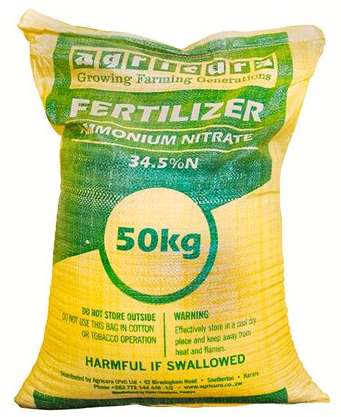
\includegraphics[width=0.6\textwidth]{Figures/ammonia/fertilizer.png}

        \column[T]{0.6\textwidth}
            \textcolor{Important}{{Ostwald process:}}
            \begin{enumerate}
                \item Producing \nitricoxide from \ammonia (Ammonia oxidation)
                \pause
                \item Producing \nitricacid from \nitricoxide
            \end{enumerate}

            \medskip
            \pause
            Why \nitricacid ?
            \begin{itemize}
                \pause
                \item Fertilizer synthesis: $\approx$ 60 million tonnes/year
                \pause
                \item TNT, mining industry
            \end{itemize}            

            \medskip
            \pause
            Other applications:
            \begin{itemize}
                \item Slip reaction, remove undesired \ammonia from industrial exhaust
                \pause
                \item Environmental reasons (\ammonia is a major air pollutant)
            \end{itemize}
            
            \medskip
            \color{Important}
                \pause
                Application → catalytic reaction tuned towards a specific product.\\
                \pause
                Selectivity → temperature, pressure, reactant ratio, type of catalyst.

    \end{columns}    
\end{frame}